\section{Công thức đánh giá chất lượng cuộc sống}
\subsection{Xây dựng công thức đánh giá chất lượng từng domain}
\subsubsection{Đánh giá theo thanh ngang}
\textbf{Giới thiệu về phương pháp:} ta sẽ dùng phương pháp cảm quan để đánh giá chất lượng của một số domain. Phương pháp này là phương pháp đánh giá chất lượng dựa trên việc sử dụng các thông tin thu được qua sự cảm nhận của các cơ quan con người khi tiếp xúc, đối mặt với các vấn đề như: thị giác, thính giác, khứu giác, xúc giác và vị giác. Các cơ quan có vai trò thu nhận các cảm giác về các chỉ tiêu chất lượng và đưa ra điểm số.\\
Để dễ hình dung hơn, nhóm mình sẽ gọi đây là phương pháp đánh giá theo thanh ngang. Chất lượng của mỗi facet được đưa ra sẽ được đánh giá theo mức điểm từ $1$ đến $100$, dựa theo bảng sau:
\begin{center}
\begin{tabular}{| m{2cm}| m{3cm} | m{2.8cm} | m{2.8cm} | m{2.8cm} | m{2.8cm}|} 
  \hline
  Cảm nhận & Rất không hài lòng & Không hài lòng &Bình thường & Hài lòng& Rất hài lòng\\ 
  \hline
  Mức điểm& $1-20$ & $21-40$ & $41-60$ & $61-80$ & $81-100$ \\ 
  \hline
\end{tabular}
\end{center}
Ta sẽ đánh giá chất lượng từng facet của mỗi domain bằng điểm số từ $1$ đến $100$. Chất lượng của domain đó sẽ là trung bình cộng chất lượng các facet được đưa ra.\\
Ưu điểm:
\begin{itemize}
    \item Hầu như không tốn chi phí.
    \item Là một trong những phương pháp đơn giản nhất.
\end{itemize}
Nhược điểm:
\begin{itemize}
    \item Mức độ chính xác không quá cao.
    \item Độ chính xác của dự đoán phụ thuộc lớn vào trình độ, kinh nghiệm, thói quen của người dự đoán.
\end{itemize}
Phương pháp đánh giá bằng thanh ngang sẽ dùng để đánh giá các domain: văn hóa xã hội, giáo dục và đào tạo, cơ sở hạ tầng. Tiếp đến nhóm mình sẽ liệt kê các facet tương ứng với mỗi domain phục vụ cho phương pháp đánh giá bằng thanh ngang này.
\subsubsection{Văn hóa xã hội}
Câu hỏi đặt ra cho chúng ta là làm sao đánh giá, đo lường được văn hóa xã hội khi nó có đặc tính vô hình, nó là một khái niệm khá trừu tượng, vốn dĩ là cái không “sờ mó” được? Dưới đây là một số yếu tố được sử dụng phổ biến nhất hiện nay để đánh giá, đo lường tác động của văn hóa đối với đời sống con người:
\subsubsubsection{Những quá trình và cấu trúc hữu hình}
Là những giá trị có thể dễ nhìn thấy, nghe thấy, cảm nhận được bao gồm:
\begin{itemize}
    \item Các thành tựu, sản phẩm truyền thống lâu đời.
    \item Lễ nghi và lễ hội hàng năm.
    \item Các biểu tượng, hình ảnh đặc trưng.
    \item Ngôn ngữ, trang phục, các trò chơi dân gian, truyền thống.
    \item Những câu chuyện, giai thoại, sử thi.
\end{itemize}
\subsubsubsection{Những giá trị được chia sẻ, được chấp nhận, được tuyên truyền}
Là những giá trị trải qua quá trình hoạt động lâu dài, được người dân, nhà nước chấp nhận, phổ biến và áp dụng bao gồm:
\begin{itemize}
    \item Những chuẩn mực hành vi. 
    \item Tập quán, tập tục.
    \item Nghi thức, tín ngưỡng.
\end{itemize}
\subsubsubsection{Những quan niệm chung}
Là những giá trị hình thành sau một thời gian hoạt  động, ghi dấu ấn vào tâm lý hầu hết các người dân và gần như không thể thay đổi, làm khác đi, trở thành điều mặc nhiên được công nhận. Chúng định hướng cho suy nghĩ, cảm nhận và hành vi của các thành viên trong cả mối quan hệ bên trong và bên ngoài gia đình và xã hội bao gồm:
\begin{itemize}
    \item Các giá trị đời sống tinh thần. 
    \item Các quan niệm, tư tưởng.
    \item Các quan niệm để phát triển.
    \item Hệ tư tưởng.
\end{itemize}
Với mỗi khía cạnh nhỏ của từng khía cạnh, ta sẽ đánh giá chất lượng của nó theo phương pháp thanh ngang. Chất lượng của từng khía cạnh sẽ là trung bình cộng chất lượng các khía cạnh nhỏ tương ứng (ví dụ như khía cạnh những giá trị được chấp nhận, được tuyên truyền gồm có những khía cạnh nhỏ là những chuẩn mực, hành vi, tập quán, tập tục và nghi thức, tín ngưỡng). Từ đó xây dựng công thức tính chất lượng của văn hóa xã hội bằng cách lấy trung bình cộng của chất lượng các khía cạnh.
\subsubsection{Giáo dục và đào tạo}
\subsubsubsection{Chương trình và chất lượng đào tạo}
\begin{itemize}
    \item Giáo viên có trình độ tốt, được tạo điều kiện để phát triển.
    \item Chương trình dạy đánh giá đúng quá trình và kết quả giáo dục.
\end{itemize}
\subsubsubsection{Phương pháp giảng dạy}
\begin{itemize}
    \item Cập nhật các phương pháp giảng dạy mới, luôn thay đổi để theo kịp với thời đại.
    \item Phương pháp giảng dạy thích hợp với người dạy và người học.
\end{itemize}
\subsubsubsection{Cơ sở vật chất}
\begin{itemize}
    \item Thiết bị công nghệ, học liệu giáo dục dễ tiếp cận.
    \item Trang bị đầy đủ các trang thiết bị phục vụ cho việc dạy học.
    \item Các trang thiết bị phải đảm bảo chất lượng tốt.
\end{itemize}
Với mỗi khía cạnh nhỏ của từng khía cạnh, ta sẽ đánh giá chất lượng của nó theo phương pháp thanh ngang. Chất lượng của từng khía cạnh sẽ là trung bình cộng chất lượng các khía cạnh nhỏ tương ứng. Từ đó xây dựng công thức tính chất lượng của giáo dục và đào tạo bằng cách lấy trung bình cộng của chất lượng các khía cạnh.
\subsubsection{Cơ sở hạ tầng}
Ta xét đến các khía cạnh của dịch vụ công, cơ sở hạ tầng
\subsubsubsection{Hệ thống điện}
\begin{itemize}
    \item Điện được cung cấp đầy đủ, ổn định, giá cả hợp lý.
\end{itemize}
\subsubsubsection{Hệ thống cấp - thoát nước}
\begin{itemize}
    \item Nước sạch được cung cấp đầy đủ, ổn định.
    \item Tiêu thoát nước dễ dàng, không gây ô nhiễm môi trường
\end{itemize}
\subsubsubsection{Hệ thống giao thông vận tải}
\begin{itemize}
    \item Đường giao thông thuận lợi, dễ dàng.
    \item Phương tiện giao thông công cộng bố trí hợp lý, thuận lợi.
    \item Không gây ô nhiễm môi trường.
\end{itemize}
\subsubsubsection{Dịch vụ viễn thông}
\begin{itemize}
    \item Dịch vụ viễn thông (điện thoại, internet) được cung cấp tốt, giá cả hợp lý.
\end{itemize}
\subsubsubsection{Dịch vụ truyền hình}
\begin{itemize}
    \item Dịch vụ truyền hình (Cable,tivi,..) được cung cấp tốt, giá cả hợp lý.
\end{itemize}
\subsubsubsection{Dịch vụ bưu chính}
\begin{itemize}
    \item Bưu kiện được gửi - nhận đầy đủ, an toàn, an ninh (bảo mật), nhanh chóng, giá cả hợp lý.
\end{itemize}
\subsubsubsection{Cơ sở giáo dục, y tế, văn hoá xã hội}
\begin{itemize}
    \item Trường học, bệnh viện và các công trình công cộng được bố trí hợp lý, thuận lợi.
\end{itemize}
Với mỗi khía cạnh nhỏ của từng khía cạnh, ta sẽ đánh giá chất lượng của nó theo phương pháp thanh ngang. Chất lượng của từng khía cạnh sẽ là trung bình cộng chất lượng các khía cạnh nhỏ tương ứng. Từ đó xây dựng công thức tính chất lượng của cơ sở hạ tầng bằng cách lấy trung bình cộng của chất lượng các khía cạnh.
\subsubsection{Môi trường tự nhiên}
Xét các yếu tố để xây dựng công thức đánh giá môi trường tự nhiên:\\
Chất lượng tiếng ồn hằng ngày: $A$\\
Gọi $B$(dB) là giá trị trung bình của tiếng ồn [11] trong 1 ngày.
\begin{itemize}
\item $B \leq 80$ là mức độ con người có thể nghe được mà không cần thiết bị bảo vệ nên $A \geq 90$\\
Từ đó ta có: $A=100-\frac{B}{8}$
\item $80 < B \leq 90$ có hại cho thính giác nếu tiếp xúc trong thời gian dài (từ 1 tiếng trở lên) nên $90 > A \geq 10$\\
Từ đó ta có: $A=100-(8B-630)$
\item $90 < B \leq 100$ rất có hại cho thính giác nếu tiếp xúc trong thời gian dài (từ 15 phút đến 1 tiếng) nên $A<10$\\
Từ đó ta có: $A=100-B$
\item $100 \leq B$ cực kì có hại, không chịu được quá 15 phút nên $A = 0$
\end{itemize}
Chất lượng bầu không khí: $C$\\
Gọi $D$ là chỉ số chất lượng không khí AQI [10] ở Việt Nam
\begin{itemize}
\item Nếu $D \leq 150$ thì $C=100-\frac{2}{3}D$
\item Nếu $D > 150$ thì $C=0$
\end{itemize}
Mức độ ảnh hưởng của thiên tai tới khu vực đang sống: $E$, được đánh giá trên thang điểm từ $0$ đến $100$.
\begin{center}
        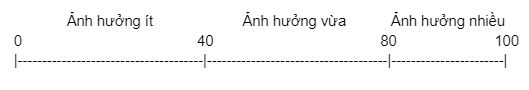
\includegraphics[scale=0.6]{2.png}
\end{center}
Từ đó ta xây dựng được công thức tính chất lượng môi trường tự nhiên là:
$$\frac{1}{3}[A + C + (100 - E)]$$
\subsubsection{An ninh quốc phòng}
Xét các yếu tố để xây dựng công thức đánh giá chất lượng an toàn, an ninh:\\
An ninh trật tự ở địa phương
\begin{itemize}
    \item Tỉ lệ trộm cắp, xảy ra mâu thuẫn ở địa phương: $A$\\
    \begin{center}
        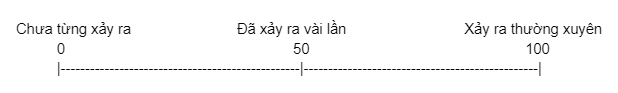
\includegraphics[scale=0.6]{1.png}
    \end{center}
    \item Tỉ lệ tệ nạn xã hội(rượu chè, cờ bạc, ma túy,..) ở địa phương: $B$\\
    \begin{center}
        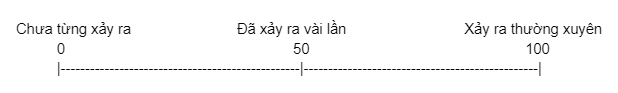
\includegraphics[scale=0.6]{1.png}
    \end{center}
\end{itemize}
An toàn giao thông
\begin{itemize}
    \item (Tỉ lệ số đèn giao thông/số nơi có giao cắt giữa các tuyến đường)x$100$: $C$
    \item Tỉ lệ biển báo giao thông ở những chỗ nguy hiểm (ngã 3, ngã 4, giao nhau với đường ưu tiên,...): $D (\%)$
    \item Tỉ lệ người không tuân thủ an toàn giao thông (vượt đèn giao thông, không đội mũ bảo hiểm, phóng nhanh, vượt ẩu,...): $E$\\
    \begin{center}
        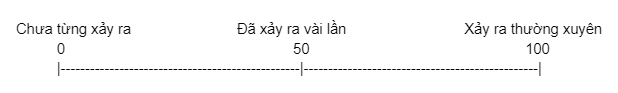
\includegraphics[scale=0.6]{1.png}
    \end{center}
\end{itemize}
Từ đó ta xây dựng được công thức tính chất lượng an toàn, an ninh chung ở địa phương:
$$\frac{1}{4}[(100 - A) + (100 - B) + C + D + (100 - E)]$$
\subsubsection{Thu nhập}
Các khoản chi tiêu trong mùa dịch [2] sẽ được chia làm hai phần chính
\subsubsubsection{Nhu cầu vật chất}
\begin{itemize}
\item Đi lại: chi phí dùng cho việc di chuyển. Vì đang trong mùa dịch nên thường mọi người sẽ hạn chế đi ra ngoài, chỉ đi bằng xe riêng của mình để đi làm hoặc mua những đồ dùng yếu phẩm. 100k/tháng (tiền xăng, bảo dưỡng, sửa xe,...).
\item Bảo vệ sức khỏe: các khoản như khám chữa bệnh, tiền thuốc, bảo hiểm y tế,... 200k/tháng.
\item Ăn, mặc, ở: quần áo, tiền ăn, tiền điện, nước,... 4000k/tháng.
\end{itemize}
\subsubsubsection{Nhu cầu văn hóa tinh thần}
\begin{itemize}
\item Học tập: học thêm, sách vở, đồ dùng học tập…. 1000k/tháng.
\item Nghỉ ngơi, giải trí: đi chơi, đi xem phim,... 500k/tháng.
\item Giao tiếp xã hội: đám tiệc, hội họp, thăm viếng,.... Vì dịch bệnh nên khoản này có thể bỏ qua.
\item Ngoài ra, phải dành một số tiền tiết kiệm, dự phòng,... chiếm $50 \%$ trong tổng số tiền chi tiêu hàng tháng.
\end{itemize}
Vậy ta có khoản chi tiêu tổng cộng trong 1 tháng là: (100k + 200k + 4000k + 1000k + 500k)/$50 \%$ = 11600k.\\
Nếu thu nhập mỗi tháng lớn hơn hoặc bằng 11600k thì chất lượng thu nhập là 100.\\
Nếu ngược lại thì chất lượng thu nhập sẽ được tính bằng công thức: (Tổng số tiền thu nhập/tổng số tiền phải chi tiêu hàng tháng)x100 = (Tổng số tiền thu nhập/11600k)x100.
\begin{nota}
$1k$ = $1000$ VND
\end{nota}
\subsubsection{Y tế và chăm sóc sức khỏe}
Để đảm bảo có sức khỏe tốt, ta cần để ý đến các yếu tố
\subsubsubsection{Chất lượng, dinh dưỡng bữa ăn và chế độ luyện tập}
Giả sử một người nam (nữ) giới trưởng thành có chiều cao, cân nặng trung bình muốn duy trì sức khoẻ hiện tại (chiều cao, cân nặng).\\ Ta có công thức tính tỷ lệ trao đổi chất cơ bản (Basal Metabolic Rate - BMR) [3]:\\
Đặt $a$ là khối lượng cơ thể theo kg, $b$ là chiều cao cơ thể theo cm, $c$ là số tuổi. Công thức được phát biểu như sau:
\begin{itemize}
\item Đối với nam giới:
$$BMR = 66,5+(13,75.a)+(5,003.b)-(6,755.c)$$
\item Đối với nữ giới: 
$$BMR=55,1+(9,563.a)+(1,850.b)-(4,676.c)$$
\end{itemize}
Chỉ số này cho ta biết mức năng lượng tối thiểu mà cơ thể cần để đảm bảo duy trì các hoạt động bình thường.
Từ đó ta có tổng lượng calories tiêu thụ/ngày: $TDEE = BMR.R$
\begin{center}
\begin{tabular}{| m{2cm}|m{2.8cm}| m{2.8cm} | m{2.8cm} | m{2.8cm} | m{2.8cm}|} 
  \hline
  Đối tượng& Ít vận động& Vận động nhẹ\newline (1-3 lần/tuần) &Vận động vừa \newline (3-5 lần/tuần) & Vận động nặng \newline (6-7 lần/tuần)& Vận động rất nặng \newline (2 lần/ngày)\\ 
  \hline
  R& $1,2$ & $1,375$ & $1,55$ & $1,725$ & $1,9$ \\ 
  \hline
\end{tabular}
\end{center}
Đặt $t = |A - TDEE|$ là lượng calo thừa hoặc thiếu đối với việc duy trì cơ thể.\\
Công thức chất lượng dinh dưỡng: $$X = (1 -\frac{t}{TDEE}).100$$
Trong đó $A$ là lượng calo nạp vào cơ thể. Chất lượng bằng $0$ nếu $t \geq TDEE$.\\
Phạm vi tin cậy [4] $95 \%$ đối với nam giới là ± $213.0$ kcal/ngày và ± $201.0$ kcal/ngày đối với phụ nữ.
\subsubsubsection{Nguồn thuốc thiết yếu}
Được đánh giá theo phương pháp thanh ngang với 2 tiêu chí
\begin{itemize}
\item Nguồn thuốc được duy trì đầy đủ, an toàn. Đặt là $Y_1$.
    \begin{center}
        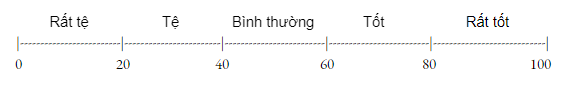
\includegraphics[scale=0.6]{3.png}
    \end{center}
\item Giá cả hợp lý. Đặt là $Y_2$
    \begin{center}
        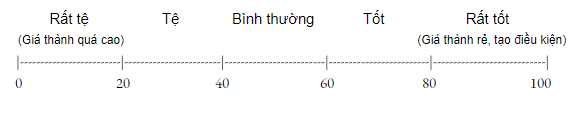
\includegraphics[scale=0.6]{4.png}
    \end{center}
\end{itemize}
Công thức đánh giá chất lượng nguồn thuốc:
$$Y = \frac{Y_1 + Y_2}{2}$$
\subsubsubsection{Vệ sinh và thu gom rác thải}
Đặt chất lượng vệ sinh và thu gom rác thải là là $Z$, ta sẽ đánh giá theo phương pháp thanh ngang với mức điểm số như sau
\begin{center}
        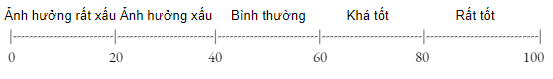
\includegraphics[scale=0.6]{5.png}
\end{center}
\subsubsubsection{Tình hình dịch bệnh ở địa phương}
Đặt chất lượng tình hình dịch bệnh ở địa phương là $T$, ta sẽ đánh giá theo phương pháp thanh ngang với mức điểm số như sau
\begin{center}
        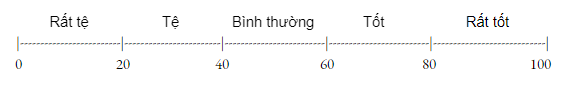
\includegraphics[scale=0.6]{3.png}
\end{center}
Ta xây dựng được công thức đánh giá chất lượng sức khỏe là
$$\frac{X + Y + Z + T}{4}$$
\subsection{Công thức đánh giá chất lượng cuộc sống}
Khi khảo sát độ quan trọng của từng domain trong bảng ở phần II, chúng mình đã thu được kết quả như sau:
\begin{center}
   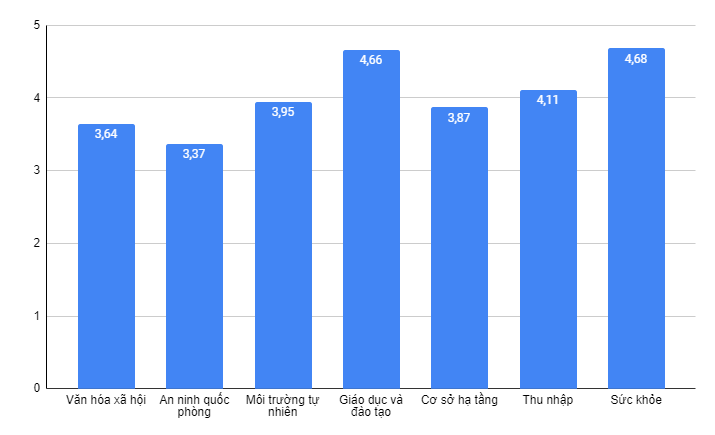
\includegraphics[scale=0.6]{6.png} 
\end{center}
Trong biểu đồ này, độ quan trọng tương ứng của từng domain là trung bình cộng của các đánh giá về độ quan trọng của domain đó, làm tròn đến $2$ chữ số thập phân.\\
Gọi chất lượng của các domain ứng với mỗi cá nhân trong biểu đồ từ trái qua phải lần lượt là $x_1, x_2,..., x_7$ với $x_i \in \mathbb{N}$, $0 \leq x_i \leq 100$. Khi đó ta xây dựng được công thức tính chất lượng cuộc sống, đặt là $X$, là:
$$X = \frac{x_1.3,64 + x_2.3,37 + x_3.3,95 + x_4.4,66 + x_5.3,87 + x_6.4,11 + x_7.4,68}{3,64 + 3,37+ 3,95+ 4,66+ 3,87 + 4,11 +4,68}$$
Công thức trên được viết lại gọn hơn là:
$$X = \frac{x_1.3,64 + x_2.3,37 + x_3.3,95 + x_4.4,66 + x_5.3,87 + x_6.4,11 + x_7.4,68}{28,28}$$
\textbf{Bảng khảo sát:} <https://bom.to/zR4QzLhqDreeVr>